%% This is an example first chapter.  You should put chapter/appendix that you
%% write into a separate file, and add a line \include{yourfilename} to
%% main.tex, where `yourfilename.tex' is the name of the chapter/appendix file.
%% You can process specific files by typing their names in at the 
%% \files=
%% prompt when you run the file main.tex through LaTeX.

\singlespacing{

\chapter{Evaluation}\label{chap:evaluation}

\section{Comparison with FEA Techniques}

\begin{figure}
  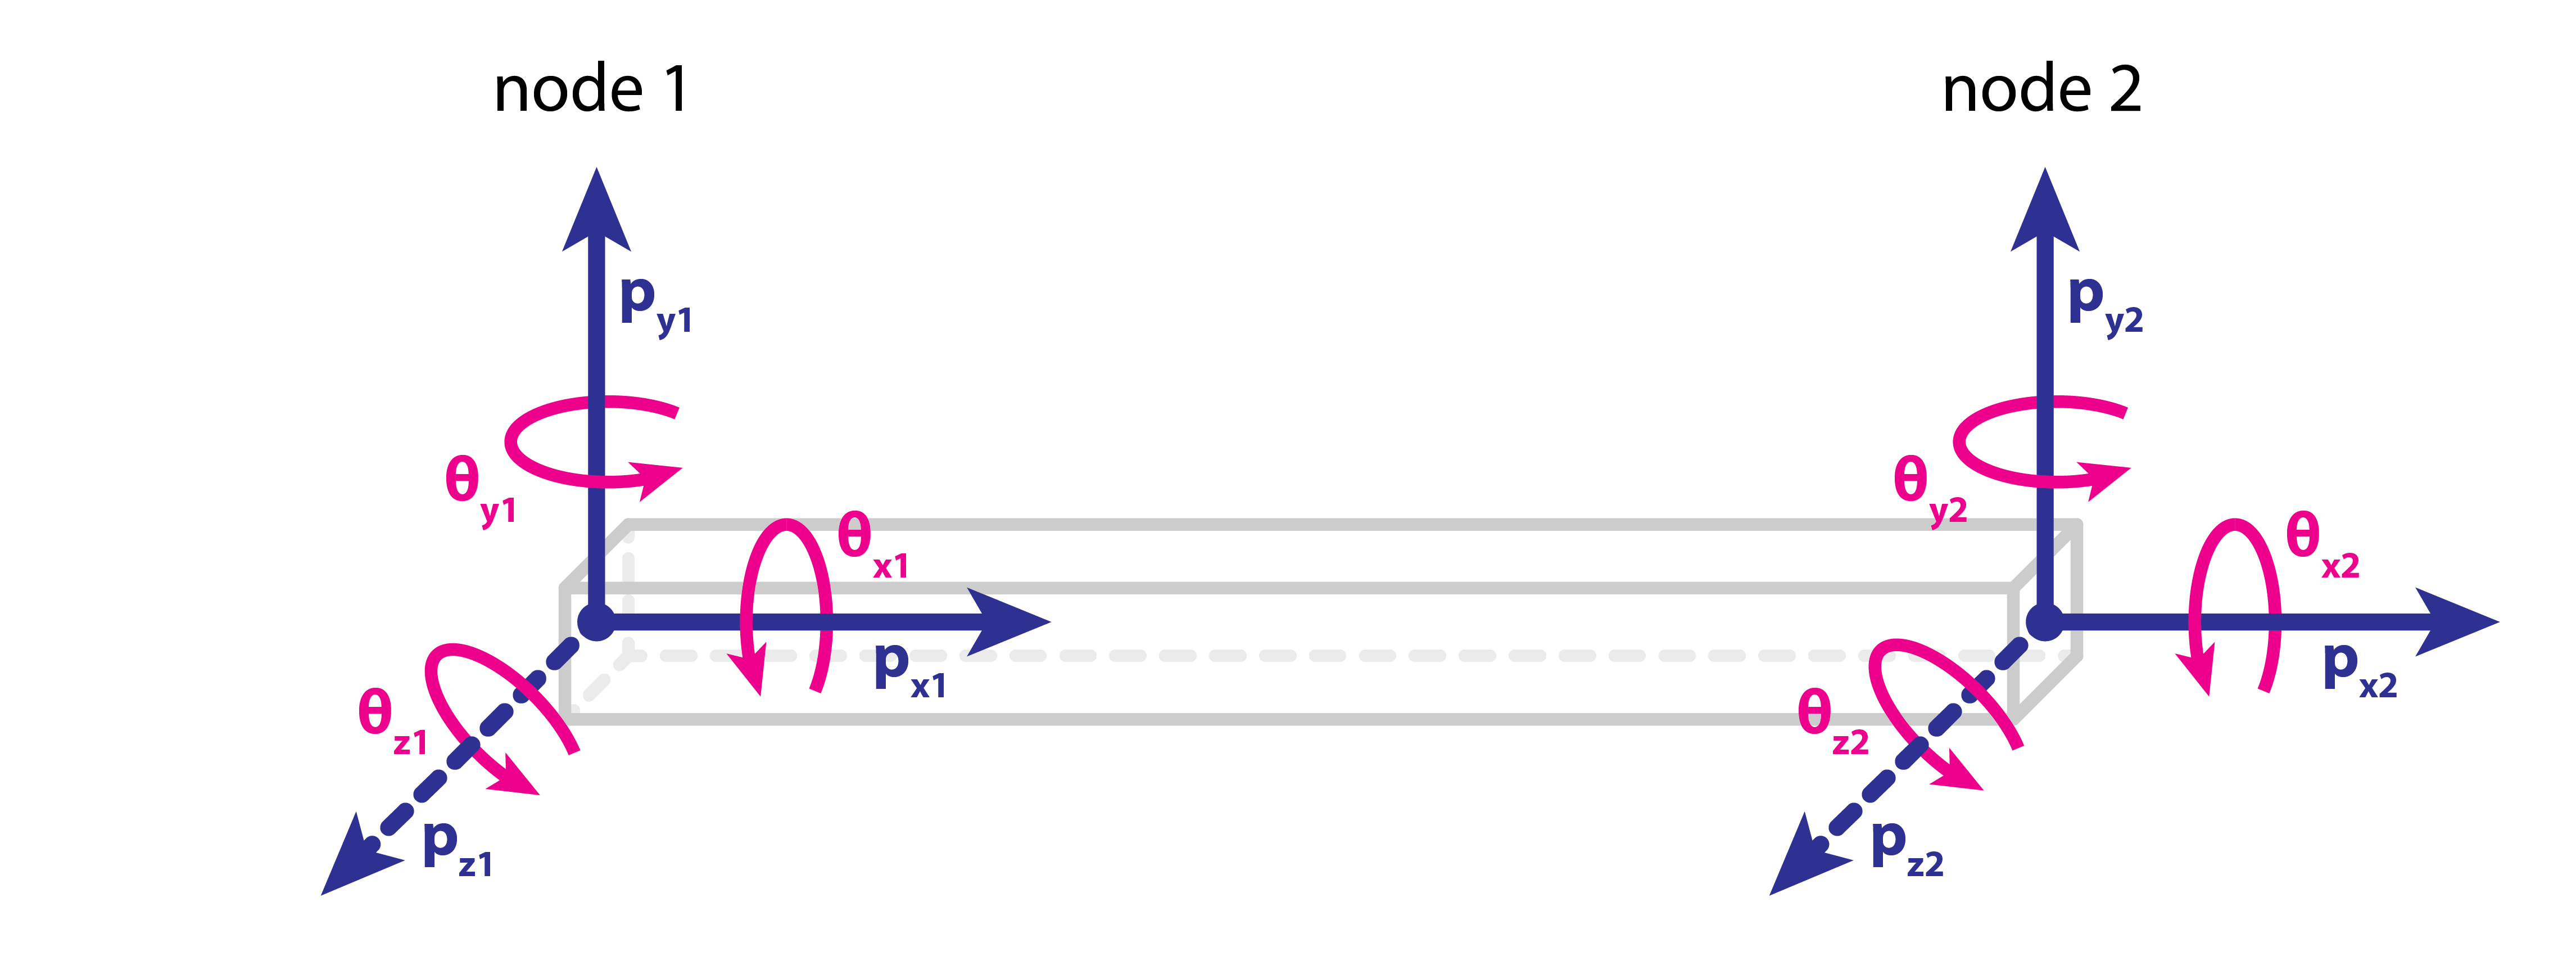
\includegraphics[width=\linewidth]{BeamSetup.png}
  \caption{Setup of 12DOF beam model connecting two nodes (nodes 1 and 2).  Translational displacement indicated by $p_x$, $p_y$, $p_z$ and angular displacement indicated by $\theta_x$, $\theta_y$, $\theta_z$.}
  \label{fig:BeamSetup}
\end{figure}

We can perform an analysis of the interactions between two cells using standard techniques from FEA to see how they compare with what we've derived in the previous sections.  Within FEA, many types of models are used to describe the behavior of linear elastic solids with varying degrees of accuracy and computational complexity.  In this analysis we'll discuss the 12DOF Timoshenko beam \cite{}.  Using this model, we can construct a beam element between two nodes that represents the material joining two adjacent cells.  The model determines the translational and rotational displaments of both nodes in 3D (Figure \ref{fig:BeamSetup}).  The Timoshenko beam element takes into account axial deformation, bending deformations in the orthogonal direction with shear effects, and torsional deformation.\\  

\textit{Shape functions} are polynomials in 1D, 2D, or 3D that describe how the behavior of the nodes should be interpolated in the regions between the nodes (e.g. the inner volume of the tetrahedron in Figure \ref{fig:TetraElement}).  Hermitian cubic shape functions are typically used for beam models; they are third order polynomials that provide continuity between discretized solutions along nodes in a beam.  A graphical description of shape functions is shown in Wolfram \cite{Wolfram2016}.  The shape functions expressed in terms of a dimensionless coordinate $\xi$ are:
\begin{align*} 
N_{x1} &= \textstyle\frac{1}{4}(1-\xi)^2(2+\xi)\\
N_{x2} &= \textstyle\frac{1}{4}(1+\xi)^2(2-\xi)\\
N_{\theta1} &= \textstyle\frac{1}{8}l(1-\xi)^2(1+\xi)\\
N_{\theta2} &= \textstyle\frac{1}{8}l(1+\xi)^2(1-\xi)
\end{align*}

where $-1 \leq \xi \leq 1$ and $\xi = -1$ at node 1 and $\xi = 1$ at node 2\\

Using these shape functions we can calculate the \textit{stiffness matrix} ($K$) of the 12DOF Timoshenko beam oriented along the x-axis:\\

\[ K =  \scriptsize {\left[ \begin{smallmatrix}
\tfrac{EA}{l} & 0 & 0 & 0 & 0 & 0 & \tfrac{-EA}{l} & 0 & 0 & 0 & 0 & 0\\
 & \tfrac{12EI_z}{l^3(1+\phi_y)} & 0 & 0 & 0 & \tfrac{6EI_z}{l^2(1+\phi_y)} & 0 & \tfrac{-12EI_z}{l^3(1+\phi_y)} & 0 & 0 & 0 & \tfrac{6EI_z}{l^2(1+\phi_y)}\\
 &  & \tfrac{12EI_y}{l^3(1+\phi_z)} & 0 & \tfrac{-6EI_y}{l^2(1+\phi_z)} & 0 & 0 & 0 & \tfrac{-12EI_y}{l^3(1+\phi_z)} & 0 & \tfrac{-6EI_y}{l^2(1+\phi_z)} & 0\\
 &  &  &  \tfrac{GJ}{l} &  0 &  0 &  0 &  0 &  0 & \tfrac{-GJ}{l} & 0 & 0\\
 &  &  &  & \tfrac{(4+\phi_z)EI_y}{l(1+\phi_z)} & 0 & 0 & 0 & \tfrac{6EI_y}{l^2(1+\phi_z)} & 0 & \tfrac{(2-\phi_z)EI_y}{l(1+\phi_z)} & 0\\
 &  &  &  &  & \tfrac{(4+\phi_y)EI_z}{l(1+\phi_y)} & 0 & \tfrac{-6EI_z}{l^2(1+\phi_y)} & 0 & 0 & 0 & \tfrac{(2-\phi_y)EI_z}{l(1+\phi_y)}\\
 &  &  &  &  &  & \tfrac{EA}{l}  & 0 & 0 & 0 & 0 & 0\\
 &  &  &  &  &  &  & \tfrac{12EI_z}{l^3(1+\phi_y)} & 0 & 0 & 0 & \tfrac{-6EI_z}{l^2(1+\phi_y)}\\
 &  &  &  &  &  &  &  & \tfrac{12EI_y}{l^3(1+\phi_z)} & 0 & \tfrac{6EI_y}{l^2(1+\phi_z)}\ & 0\\
 &  & symmetric &  &  &  &  &  &  & \tfrac{GJ}{l} & 0 & 0\\
 &  &  &  &  &  &  &  &  &  & \tfrac{(4+\phi_z)EI_y}{l(1+\phi_z)} & 0\\
  &  &  &  &  &  &  &  &  &  &  & \tfrac{(4+\phi_y)EI_z}{l(1+\phi_y)}\\
 \end{smallmatrix} \right] }\]
 
 where
\[ \phi_y = \dfrac{12EI_z}{GA_{sy}l^2} \qquad  \textrm{and} \qquad \phi_z = \dfrac{12EI_y}{GA_{sz}l^2} \]


The stiffness matrix gives us a way to convert between translational/rotational nodal displacements and forces, according to the following equation:

 \begin{equation} \label{eq:forcestiffnessdisp} \vec{F} = -K\vec{u} \end{equation}
where:
\[ \vec{F} =  \left[ \begin{array}{ccc}
F_{x1}\\
F_{y1}\\
F_{z1}\\
T_{x1}\\
T_{y1}\\
T_{z1}\\
F_{x2}\\
F_{y2}\\
F_{z2}\\
T_{x2}\\
T_{y2}\\
T_{z2}
 \end{array} \right]  \qquad \qquad  
 \vec{u} =  \left[ \begin{array}{ccc}
p_{x1}\\
p_{y1}\\
p_{z1}\\
\theta_{x1}\\
\theta_{y1}\\
\theta_{z1}\\
p_{x2}\\
p_{y2}\\
p_{z2}\\
\theta_{x2}\\
\theta_{y2}\\
\theta_{z2}
 \end{array} \right]
 \]\\
 
where $F_1$, $F_2$ are translational forces acting on nodes 1 and 2, $T$ are torques, $p$ are translational displacements, and $\theta$ are rotational displacements.  The negative sign was put in front of the stiffness matrix to keep the same convention of restoring forces used in Chapter \ref{chap:functionSim}.\\

Multiplying through Equation \ref{eq:forcestiffnessdisp} gives us 12 equations:

\begin{subequations}
\begin{align} 
\label{eq:fx1}
F_{x1} &=  -\dfrac{EA}{l}p_{x1} + \dfrac{EA}{l}p_{x2} \\[10pt]
\label{eq:fy1}
F_{y1} &=  -\dfrac{12EI_z}{l^3(1+\phi_y)}p_{y1} - \dfrac{6EI_z}{l^2(1+\phi_y)}\theta_{z1} + \dfrac{12EI_z}{l^3(1+\phi_y)}p_{y2} - \dfrac{6EI_z}{l^2(1+\phi_y)}\theta_{z2}\\[10pt]
\label{eq:fz1}
F_{z1} &=  -\dfrac{12EI_y}{l^3(1+\phi_z)}p_{z1} - \dfrac{6EI_y}{l^2(1+\phi_z)}\theta_{y1} + \dfrac{12EI_y}{l^3(1+\phi_z)}p_{z2} - \dfrac{6EI_y}{l^2(1+\phi_z)}\theta_{y2}\\[10pt]
\label{eq:tx1}
T_{x1} &=  -\dfrac{GJ}{l}\theta_{x1} + \dfrac{GJ}{l}\theta_{x2} \\[10pt]
\label{eq:ty1}
T_{y1} &= \dfrac{6EI_y}{l^2(1+\phi_z)}p_{z1} - \dfrac{(4+\phi_z)EI_y}{l(1+\phi_z)}\theta_{y1}  - \dfrac{6EI_y}{l^2(1+\phi_z)}p_{z2} - \dfrac{(2-\phi_z)EI_y}{l(1+\phi_z)}\theta_{y2} \\[10pt]
\label{eq:tz1}
T_{z1} &=  -\dfrac{6EI_z}{l^2(1+\phi_y)}p_{y1} - \dfrac{(4+\phi_y)EI_z}{l(1+\phi_y)}\theta_{z1}  + \dfrac{6EI_z}{l^2(1+\phi_y)}p_{y2} - \dfrac{(2-\phi_y)EI_z}{l(1+\phi_y)}\theta_{z2} \\[10pt]
\label{eq:fx2}
F_{x2} &=  -F_{x1}\\[10pt]
\label{eq:fy2}
F_{y2} &=  -F_{y1}\\[10pt]
\label{eq:fz2}
F_{z2} &=  -F_{z1}\\[10pt]
\label{eq:tx2}
T_{x2} &=  -T_{x1}\\[10pt]
\label{eq:ty2}
T_{y2} &=  \dfrac{6EI_y}{l^2(1+\phi_z)}p_{z1} - \dfrac{(2-\phi_z)EI_y}{l(1+\phi_z)}\theta_{y1}  - \dfrac{6EI_y}{l^2(1+\phi_z)}p_{z2} - \dfrac{(4+\phi_z)EI_y}{l(1+\phi_z)}\theta_{y2} \\[10pt]
\label{eq:tz2}
T_{z2} &= -\dfrac{6EI_z}{l^2(1+\phi_y)}p_{y1} - \dfrac{(2-\phi_y)EI_z}{l(1+\phi_y)}\theta_{z1}  + \dfrac{6EI_z}{l^2(1+\phi_y)}p_{y2} - \dfrac{(4+\phi_y)EI_z}{l(1+\phi_y)}\theta_{z2}
\end{align}
\end{subequations}\\

Combining Equations \ref{eq:fx1} and \ref{eq:kaxial} gives us the x-axis spring component of Equation \ref{eq:translationalEqOpp}, assuming no relative rotation between the nodes:
\[F_{x1} =  k_{axial_x}(p_{x2} - p_{x1}) \]

Equations \ref{eq:fy1} and \ref{eq:fz1} have the same general form.  Rearranging Equation \ref{eq:fy1} gives:
\begin{equation}\label{eq:Fy1decomp}
 F_{y1} =  \dfrac{12EI_z}{l^3(1+\phi_y)} (p_{y2} -p_{y1}) - \dfrac{6EI_z}{l^2(1+\phi_y)}(\theta_{z1} + \theta_{z2}) 
 \end{equation}

The force $F_{y1}$ acting on node 1 is a combination of contributions from bending and shear stiffnesses.  Assuming shear dominance, we can reduce Equation \ref{eq:Fy1decomp} to:
\[ F_{y1} =  \dfrac{12EI_z}{l^3\phi_y} (p_{y2} -p_{y1}) - \dfrac{6EI_z}{l^2\phi_y}(\theta_{z1} + \theta_{z2}) 
\]
\[ F_{y1} =  \dfrac{GA_{sy}}{l} (p_{y2} -p_{y1}) - \dfrac{GA_{sy}}{2}(\theta_{z1} + \theta_{z2}) 
\]

Substituting Equation \ref{eq:kshear} gives:

\[ F_{y1} =  k_{shear_{xy}} (p_{y2} -p_{y1}) - k_{shear_{xy}}l\dfrac{(\theta_{z1} + \theta_{z2})}{2}
\]

\[ F_{y1} =  k_{shear_{xy}} (p_{y2} -p_{y1} - l\theta_{z_{avg}})
\]

Which is a	 small angle approximation of the y-axis spring component of Equation \ref{eq:translationalEqOpp}.\\

We'll account for the bending dominant form of Equation \ref{eq:Fy1decomp} in Section \ref{sec:bendingdominance}.\\

As discussed in Equation \ref{eq:translationalEqOpp}, the translational forces acting on node 1 are equal and opposite those acting on node 2.  This is summed up by Equations \ref{eq:fx2}, \ref{eq:fy2}, and \ref{eq:fz2}.\\

Combining Equations \ref{eq:tz1} and \ref{eq:ktorsion} gives us a small angle approximation to the x-axis rotational component of Equation \ref{eq:T1verbose} (in this case the small angle approximation reduces the first term of Equation \ref{eq:T1verbose} to zero, assuming that torques applied to node1 by node 2 have no x component):
\[T_{x1} =  k_{torsion_x}(\theta_{x2} - \theta_{x1}) \]

Equations \ref{eq:ty1} and \ref{eq:tz1} have the same general form.  Rearranging Equation \ref{eq:ty1} gives:
\begin{equation}\label{eq:Ty1decomp}
T_{y1} = - \dfrac{6EI_y}{l^2(1+\phi_z)}(p_{z2}- p_{z1}) - \dfrac{EI_y}{l(1+\phi_z)}((4+\phi_z)\theta_{y1}  + (2-\phi_z)\theta_{y2})
\end{equation}

As with Equation \ref{eq:Fy1decomp}, this is a combination of shear and bending effects.  Assuming shearing dominance \ref{eq:Ty1decomp} reduces to:
\begin{equation}\label{eq:Ty1decomp2}
T_{y1} = - \dfrac{6EI_y}{l^2\phi_z}(p_{z2}- p_{z1}) - \dfrac{EI_y}{l}(\theta_{y1}  - \theta_{y2})
\end{equation}

\[T_{y1} = - \dfrac{GA_{sz}}{2}(p_{z2}- p_{z1}) + \dfrac{EI_y}{l}(\theta_{y2}  - \theta_{y1})\]

Substituting Equation \ref{eq:kshear} and \ref{eq:kbending} gives:
\[T_{y1} = \dfrac{-l}{2}k_{shear_{xz}}(p_{z2}- p_{z1}) + k_{bending_y}(\theta_{y2}  - \theta_{y1})\]

which is a small angle approximation of the y-component of \ref{eq:T1verbose} with:
\[ \vec{l}_{rot12} \approx \vec{l}_{nom12} = \left[ \begin{array}{ccc}
-l\\
0\\
0
 \end{array} \right]\]
 
Following this same procedure with Equation \ref{eq:tz1} gives a similar result, but with an extra negative sign:
\[T_{z1} = (-)\dfrac{-l}{2}k_{shear_{xy}}(p_{y2}- p_{y1}) + k_{bending_z}(\theta_{z2}  - \theta_{z1})\]
 
This negative is a byproduct of the crossproduct in Equation \ref{eq:T1verbose}, according to the following unit vector relationships:
\begin{equation}\label{eq:crossUnits}
\hat{x} \times \hat{y} = \hat{z}  \qquad \hat{x} \times \hat{z} = -\hat{y}  
\end{equation}

We'll account for the bending dominant form of Equation \ref{eq:Ty1decomp} in Section \ref{sec:bendingdominance}.\\

Finally, Equation \ref{eq:ty2} and \ref{eq:tz2} have the same general form. Rearranging Equation \ref{eq:ty2} gives:
\begin{equation}\label{eq:Ty2Decomp}
T_{y2} =  -\dfrac{6EI_y}{l^2(1+\phi_z)}(p_{z2} - p_{z1}) - \dfrac{EI_y}{l(1+\phi_z)}((2-\phi_z)\theta_{y1}  + (4+\phi_z)\theta_{y2})
\end{equation}

In the case of shearing dominance, \ref{eq:Ty2Decomp} reduces to:
\[  T_{y2} =  -\dfrac{6EI_y}{l^2\phi_z}(p_{z2} - p_{z1}) - \dfrac{EI_y}{l}(\theta_{y2}  - \theta_{y1}) \]

\[  T_{y2} =  \dfrac{GA_{sz}}{2}(p_{z1} - p_{z2}) + \dfrac{EI_y}{l}(\theta_{y1}  - \theta_{y2}) \]

Substituting Equation \ref{eq:kshear} and \ref{eq:kbending} gives:
\[  T_{y2} =  \dfrac{l}{2}k_{shear_{xz}}(p_{z1} - p_{z2}) + k_{bending_y}(\theta_{y1}  - \theta_{y2}) \]

which is a small angle approximation of the y-component of \ref{eq:T2verbose} with:
\[ \vec{l}_{rot21} \approx \vec{l}_{nom21} = \left[ \begin{array}{ccc}
l\\
0\\
0
 \end{array} \right]\]

Following this same procedure with \ref{eq:tz2}, we get:
\[  T_{y2} =  (-)\dfrac{l}{2}k_{shear_{xy}}(p_{y1} - p_{y2}) + k_{bending_z}(\theta_{z1}  - \theta_{z2}) \]

where again, the extra negative sign is accounted for by the cross product in Equation \ref{eq:T2verbose} and the relationships \ref{eq:crossUnits}.\\

Again, we'll account for the bending dominant form of Equation \ref{eq:Ty2Decomp} in Section \ref{sec:bendingdominance}.

\subsection{Accounting for Bending Dominance}\label{sec:bendingdominance}

Assuming  bending dominance, we can reduce Equation \ref{eq:Fy1decomp} to:
\[ F_{y1} =  \dfrac{12EI_z}{l^3} (p_{y2} -p_{y1}) - \dfrac{6EI_z}{l^2}(\theta_{z1} + \theta_{z2})  \]
\[ F_{y1} =  \dfrac{12EI_z}{l^3} (p_{y2} -p_{y1}) - \dfrac{12EI_z}{l^3}(l\theta_{avg})  \]
\[ F_{y1} =  \dfrac{12EI_z}{l^3} (p_{y2} -p_{y1} - l\theta_{avg})  \]

Assuming bending dominance, \ref{eq:Ty1decomp} reduces to:
\[T_{y1} = - \dfrac{6EI_y}{l^2}(p_{z2}- p_{z1}) - \dfrac{2EI_y}{l}(2\theta_{y1}  + \theta_{y2})\]


\section{Comparison with VoxCAD Physics Engine}

Removing the shear terms from elements of the 12DOF Timoshenko model leaves us with an Euler-Bernoulli beam element.  This model assumes no shearing of a beam element joining two cells.  For a beam oriented along the x-axis, using the same Hermitian cubic shape functions, we get the following stiffness matrix:

\[ K =  \small {\left[ \begin{smallmatrix}
\tfrac{EA}{l} & 0 & 0 & 0 & 0 & 0 & \tfrac{-EA}{l} & 0 & 0 & 0 & 0 & 0\\
 & \tfrac{12EI_z}{l^3} & 0 & 0 & 0 & \tfrac{6EI_z}{l^2} & 0 & \tfrac{-12EI_z}{l^3} & 0 & 0 & 0 & \tfrac{6EI_z}{l^2}\\
 &  & \tfrac{12EI_y}{l^3} & 0 & \tfrac{-6EI_y}{l^2} & 0 & 0 & 0 & \tfrac{-12EI_y}{l^3} & 0 & \tfrac{-6EI_y}{l^2} & 0\\
 &  &  &  \tfrac{GJ}{l} &  0 &  0 &  0 &  0 &  0 & \tfrac{-GJ}{l} & 0 & 0\\
 &  &  &  & \tfrac{4EI_y}{l} & 0 & 0 & 0 & \tfrac{6EI_y}{l^2} & 0 & \tfrac{EI_y}{l} & 0\\
 &  &  &  &  & \tfrac{4EI_z}{l} & 0 & \tfrac{-6EI_z}{l^2} & 0 & 0 & 0 & \tfrac{EI_z}{l}\\
 &  &  &  &  &  & \tfrac{EA}{l}  & 0 & 0 & 0 & 0 & 0\\
 &  &  &  &  &  &  & \tfrac{12EI_z}{l^3} & 0 & 0 & 0 & \tfrac{-6EI_z}{l^2}\\
 &  &  &  &  &  &  &  & \tfrac{12EI_y}{l^3} & 0 & \tfrac{6EI_y}{l^2}\ & 0\\
 &  & symmetric &  &  &  &  &  &  & \tfrac{GJ}{l} & 0 & 0\\
 &  &  &  &  &  &  &  &  &  & \tfrac{4EI_y}{l} & 0\\
  &  &  &  &  &  &  &  &  &  &  & \tfrac{4EI_z}{l}\\
 \end{smallmatrix} \right] } \]
 
 Multiplying through Equation \ref{eq:forcestiffnessdisp} gives us 12 equations:

\begin{subequations}
\begin{align} 
\label{eq:fx1vox}
F_{x1} &=  \dfrac{EA}{l}p_{x1} - \dfrac{EA}{l}p_{x2} \\[10pt]
\label{eq:fy1vox}
F_{y1} &=  \dfrac{12EI_z}{l^3}p_{y1} + \dfrac{6EI_z}{l^2}\theta_{z1} - \dfrac{12EI_z}{l^3}p_{y2} + \dfrac{6EI_z}{l^2}\theta_{z2}\\[10pt]
\label{eq:fz1vox}
F_{z1} &=  \dfrac{12EI_y}{l^3}p_{z1} - \dfrac{6EI_y}{l^2}\theta_{y1} - \dfrac{12EI_y}{l^3}p_{z2} - \dfrac{6EI_y}{l^2}\theta_{y2}\\[10pt]
\label{eq:tx1vox}
T_{x1} &=  \dfrac{GJ}{l}\theta_{x1} - \dfrac{GJ}{l}\theta_{x2} \\[10pt]
\label{eq:ty1vox}
T_{y1} &= - \dfrac{6EI_y}{l^2}p_{z1} + \dfrac{4EI_y}{l}\theta_{y1}  + \dfrac{6EI_y}{l^2}p_{z2} + \dfrac{2EI_y}{l}\theta_{y2} \\[10pt]
\label{eq:tz1vox}
T_{z1} &=  \dfrac{6EI_z}{l^2}p_{y1} + \dfrac{(4EI_z}{l}\theta_{z1}  - \dfrac{6EI_z}{l^2}p_{y2} + \dfrac{2EI_z}{l}\theta_{z2} \\[10pt]
\label{eq:fx2vox}
F_{x2} &=  -F_{x1}\\[10pt]
\label{eq:fy2vox}
F_{y2} &=  -F_{y1}\\[10pt]
\label{eq:fz2vox}
F_{z2} &=  -F_{z1}\\[10pt]
\label{eq:tx2vox}
T_{x2} &=  -T_{x1}\\[10pt]
\label{eq:ty2vox}
T_{y2} &=  - \dfrac{6EI_y}{l^2}p_{z1} + \dfrac{2EI_y}{l}\theta_{y1}  + \dfrac{6EI_y}{l^2}p_{z2} + \dfrac{4EI_y}{l}\theta_{y2} \\[10pt]
\label{eq:tz2vox}
T_{z2} &= \dfrac{6EI_z}{l^2}p_{y1} + \dfrac{2EI_z}{l}\theta_{z1}  - \dfrac{6EI_z}{l^2}p_{y2} + \dfrac{4EI_z}{l}\theta_{z2}
\end{align}
\end{subequations}\\

Following the same logic as the Timoshenko model, it can be shown that this is equivalent to a small angle approximation of the equations derived in Chapter \ref{chap:functionSim}, minus the contribution from shear.

\section{Comparison with COMSOL Simulation}



\section{Performance Metrics}
